\documentclass{article}
\usepackage[utf8]{inputenc}
\usepackage[T1]{fontenc} 
\usepackage[slovene]{babel} 

\usepackage{enumitem} 
\usepackage{hyperref}
\usepackage{amsmath}
\usepackage{amsthm} 
\usepackage{amssymb}
\usepackage{lmodern}
\usepackage{amsfonts} 
\usepackage{mathtools}
\usepackage{graphicx}
\usepackage{float}
\usepackage{dsfont}
\usepackage{arydshln}

\DeclareMathOperator{\EX}{\mathbb{E}}
%\setlength{\abovecaptionskip}{15pt plus 3pt minus 2pt}

\begin{document}

\title{Projekt statistika\\
    \large Projekt pri predmetu Statistika
}
\author{
    Matej Novoselec\\
}
\date{30.\ junij 2023}

\maketitle
\pagebreak

\section{Kibergrad}
Podani so nam podatki o dohodkih $43886$ družin iz mesta Kibergrad. Podatke o dohodkih bomo analizirali v odvisnosti od tipa družin, ki je posredovala podatke. 
Pri obdelavi podatkov si bomo pomagali z datoteko $statistika\_naloga\_1.py$, ki je namenjena predvsem izrisu grafov, ter numeričnim izračunom željenih vrednosti, prek danih podatkov. 
\newline
Družine razdelimo v $3$ tipe: tip 1 - družina z zakonskima ali zunajzakonskima partnerjema, tip 2 - enostarševska družina z očetom, tip 3 - enostarševska družina z materjo.
Imamo 33403 podatkov od družin tipa 1, 2054 podatkov od družin tipa 2 in 8429 podatkov od družin tipa 3.
Za vsak tip družine izberemo enostaven slučajen vzorec velikosti $500$ in narišemo pripadajočo škatlo z brki.

\begin{figure}[H]
    \begin{center}
    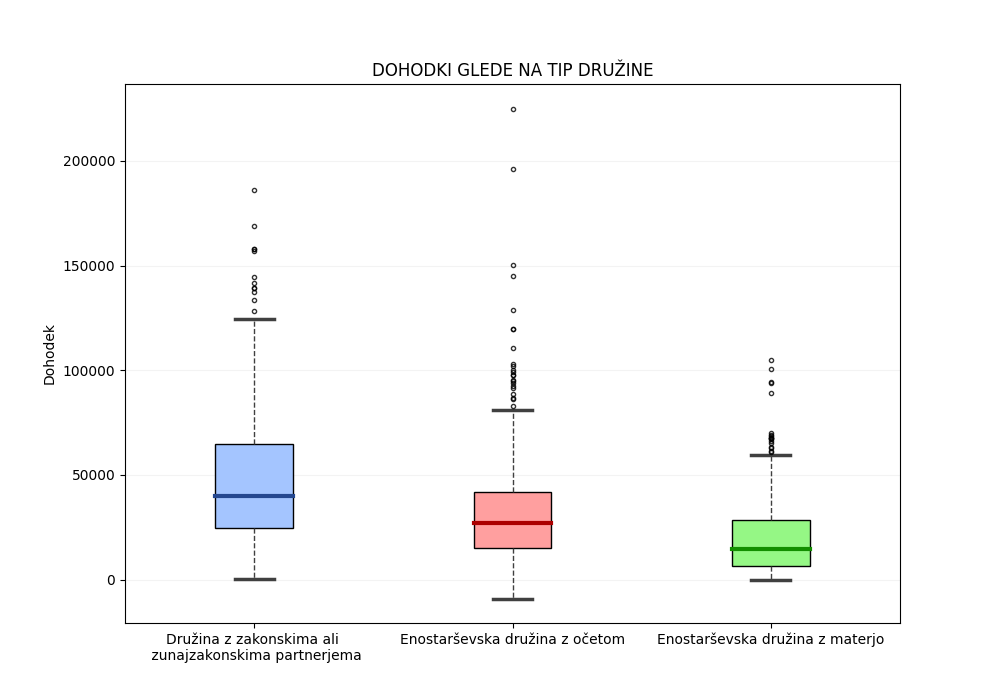
\includegraphics[width=\linewidth]{naloga1a.png}
    \vspace*{-10mm}\caption{Škatle z brki za dohodke različnih tipov družin}
    \end{center}    
\end{figure}

Hitro vidimo, da so vrednosti prvega, drugega in tretjega kvantila pri družinah tipa 1 (družinah z zakonskima ali zunajzakonskima partnerjema) višji od prvega, drugega in tretjega kvantila pri družinah tipa 2 in tipa 3. 
Iz tega lahko sklepamo, da so  povprečju dohodki omenjenega tipa družin večji od obeh ostalih tipov. Na podoben način lahko sklepamo tudi, da so dohodki v enostarševski družini z očetom v povprečju nekoliko višji od dohodkov enostarševskih družin z materjo. 
Opazimo tudi, da je varianca dohodkov pri družinah tipa 1 večja od variance podatkov o dohodkih družin preostalih tipov. 
Osamelcev opazimo največ pri družinah tipa 2, podatki pri družinah tipa 3 pa so najmanj razpršeni. 
Vredno je omeniti tudi, da je pri družinah tipa 1 in tipa 3 porazdelitev dohodkov nekoliko nagnjena k dohodkov višje vrednosti.
\newline
Povzeli bi lahko, da nekoliko izstopajo podatki o družinah tipa 1, ki imajo povprečno najvišji dohodek, a imajo obenem tudi veliko varianco, njihova porazdelitev pa je nagnjena k višjim vrednostim.
Vseeno moramo biti s sklepanjem nekoliko pazljivi, saj je vzorec velikosti $500$ za $33403$ podatkov relativno majhen.
\newline
\newline
Sedaj se osredotočimo na družine tipa 1 in iz podatkov izberimo še štiri enostavne slučajne vzorce. 
Opažanja so prikazana z vzporednimi škatlami z brki, pri čemer temnejše obarvana škatla z brki pripada podatkom, ki so bili izbrani kot enostavni slučajni vzorec za družine tega tipa iz prejšne podnaloge.

\begin{figure}[H]
    \begin{center}
    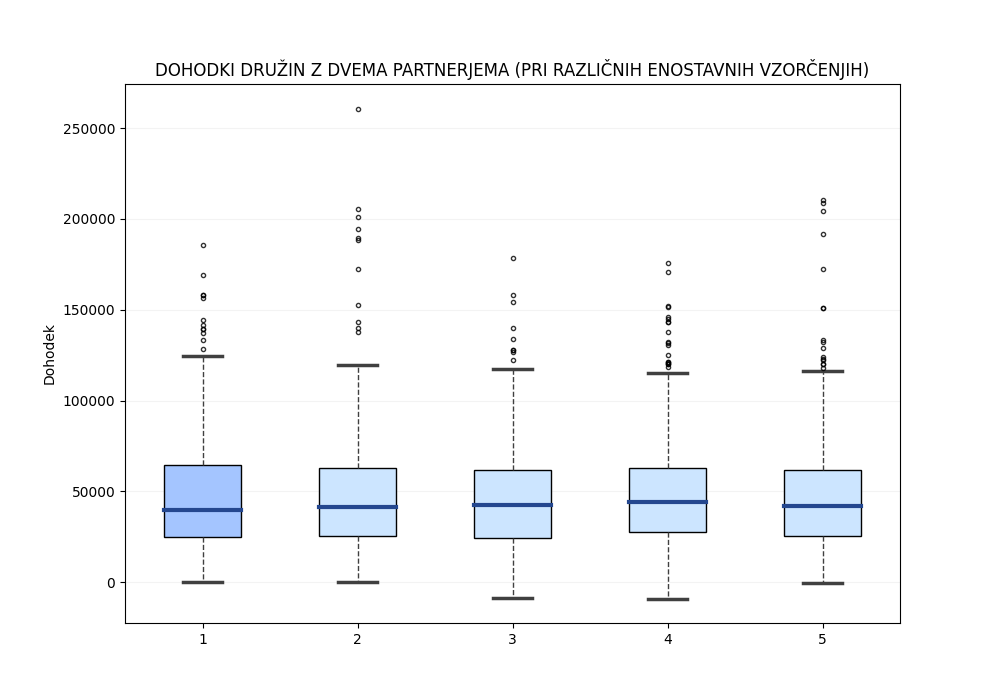
\includegraphics[width=\linewidth]{naloga1b.png}
    \vspace*{-10mm}\caption{Škatle z brki za dohodke družin z dvema partnerjema}
    \end{center}    
\end{figure}

Opazimo, da je bil zgoraj izbrani vzorec, kljub temu, da je bil dokaj majhen glede na število vseh podatkov, v veliki meri (vsaj iz vidika ostalih štirih vzorcev) representativen.
Vidno je namreč, da so vrednosti prvega in tretjega kvantila pri vzorcih dokaj usklajeni. 
Tudi iz vidika števila osamelcev je prvotno izbran vzorec representativen. 
Nekoliko se od representativnosti odmaknemo le pri vrednosti drugega kvantila, ki je pri našem vzorcu nekoliko nižje kot pri ostalih, posledično pa so podatki o dohodkih prvotno izbranega vzorca nekoliko nagnjeni k višjim vrednostim.
\newline
\newline
Zadnje podnaloge se za začetek lotimo nekoliko bolj teoretično, ter šele nato vstavimo podatke za izračun željenih vrednosti. 
Z $n$ označimo število vseh numeričnim podatkov, t.j. skupni numerus je enak $n$. Podatki so razdeljeni v skupine (glede na tip družine), $n_i$ naj označuje število podatkov za skupino s tipom družine $i$ ($i$ seveda tu $1,~2~\text{ali}~3$).
Definirajmo še uteži za posamezno skupino, kot $w_i = n_i/n$.
\newline
Pričakovano vrednost za celoten Kibergrad lahko izrazimo prek pričakovanih vrednosti za posamezne skupine (označimo jih z $\mu_i$) kot:
$$
    \mu = w_1 \mu_1 + w_2 \mu_2 + w_3 \mu_3.
$$
Če z $\sigma_{i}^2$ označimo varianco znotraj $i$-te skupine, lahko na podoben način varianco dohodka za celoten Kibergrad izrazimo kot:
$$
\sigma^2 = \sigma_{P}^2 + \sigma_{N}^2,~~~\text{kjer:}~~\sigma_{P}^2 = \sum_{i=1}^{3}{w_i(\mu_i - \mu)^2}~~~\text{in}~~~\sigma_{N}^2 = \sum_{i=1}^{3}{w_i \sigma_{i}^2}.
$$
Izpeljava je navedena v \cite{poj_nepo_var}. V zgornjem zapisu $\sigma_P^2$ označuje s tipom družine pojasnjeno varianco, $\sigma_N^2$ pa nepojasnjeno varianco. Naloga nas sprašuje po obeh. 
\newline
Numerično v $python$ datoteki poračunamo približke za pričakovane vrednosti in variance za posamezne skupini, ter po zgoraj zapisanih formulah dobimo, 
da s tipom družine pojasnjena varianca znaša $113781161.94$, nepojasnjena varianca pa $912604507.95$. Omenimo še, da delež pojasnjene variance ($\eta^2 = \frac{\sigma_{P}^2}{\sigma^2}$) znaša $0.11085$, pojasnjeni standardni odklon pa $10666.83$.
\newline
\newline
Oglejmo si novo pridobljene podatke v luči preteklih opažanj, predvsem iz vidika povprečnih dohodkov različnim tipov družin. Že v komentarju prve podnaloge smo omenili, da so med povprečnimi dohodki tipov družin opazne razlike.  
Sedaj opazimo, da je tudi vrednost pojasnjenega standardnega odklona visoka glede na povprečne dohodke posameznih tipov družin (te znašajo $47187.48$ za tip 1, $31637.36$ za tip 2 in $20508.19$ za tip 3), kar dodatno nakazuje na razlike med povprečnimi dohodki posameznih tipov družin.
Vrednost deleža pojasnjene variance le dodatno potrdi že zapisano.

\pagebreak

\section{Kromatin}
Vredno je zapisati nekoliko bolj matematično interpretacijo problema/navodila. 
Podatki pripadajo trem različnim eksperimentom (podatki so ločeni glede na dolžino opazovanega Kromatina), ki bodo določali končne vrednosti in rezultate, a so problemi, ki jih podajajo, teoretično iste narave. 
Za podan problem sedaj razvijemo teoretični pristop in se lotimo reševanja podnaloge a) in b). 
\newline
Imamo $n$ neodvisnih, enako porazdeljenih slučajnih spremenljivk, označimo jih z $R_1,~R_2,~\dots,~R_n$. 
Porazdeljene naj bodo Rayleighovo, t.j. z gostoto:
$$
f_{R_i}(r_{i} \mid \theta)=\left\{\begin{array}{cl}
\frac{r_i}{\theta^{2}} \exp \left(-\frac{r_{i}^{2}}{2 \theta^{2}}\right) & ;~~r>0 \\
0 & ;~~\text{sicer }
\end{array}\right. .
$$
Zaradi predpostavljene neodvisnosti, je potem $(R_1,~R_2,~\dots,~R_n)$ porazdeljen z gostoto:
$$
    \prod_{i=1}^{n}{f_{R_i}(r_{i} \mid \theta)} = 
    \bigg(\frac{1}{\theta^{2n}}\prod_{i=1}^{n}{r_i}\bigg) \exp\bigg(-\frac{1}{2 \theta^{2}} \sum_{i=1}^{n}{r_i^2}\bigg);~~r_i>0.
$$
Lotimo se podnaloge a). Velja:
$$
L(\theta \mid (r_1,~r_2,~\dots,~r_n)) = \prod_{i=1}^{n}{L_i(\theta \mid r_i)} = \prod_{i=1}^{n}{f_{R_i}(r_i \mid \theta)}
$$
in
$$
l(\theta \mid (r_1,~r_2,~\dots,~r_n)) = \ln L(\theta \mid (r_1,~r_2,~\dots,~r_n)) = \sum_{i=1}^{n}{\ln \big(f_{R_i}(r_i \mid \theta)\big)}, 
$$
ter zato:
$$
l(\theta \mid (r_1,~r_2,~\dots,~r_n)) = -2n \ln(\theta) + \sum_{i=1}^{n}{\ln(r_i)} - \frac{1}{2\theta^2} \sum_{i=1}^{n}{r_i^2}~.
$$
Iščemo cenilko za $\theta$ po metodi največjega verjetja, zato si ogledamo enakost:
$$
0 = \frac{\partial l(\theta \mid (r_1,~\dots,~r_n))}{\partial \theta} = - \frac{2n}{\theta} + \frac{1}{\theta^3}\sum_{i=1}^{n}{r_i^2}.
$$
Za cenilko po metodi največjega verjetja tako dobimo:
$$
\hat{\theta}_{MNV} = \sqrt{\frac{1}{2n}{\sum_{i=1}^{n}{r_i^2}}}~.
$$
Za rešitev podnaloge b) si oglejmo pričakovano vrednost (Rayleighove) slučajne spremenljivke $R$:
$$
\EX(R) = \int_{0}^{\infty}{r~f(r \mid \theta)~dr}= \int_{0}^{\infty}{\frac{r^2}{\theta^{2}}~\exp\Big(-\frac{r^{2}}{2 \theta^{2}}\Big)~dr}.
$$
V integral uvedemo $\tau = \frac{r^{2}}{2 \theta^{2}}$ in dobimo
$$
\EX(R) = \int_{0}^{\infty}{\sqrt{2 \tau}~\theta ~e^{-\tau}~ d \tau} = \theta \sqrt{2}\int_{0}^{\infty}{\tau^{1/2}~e^{-\tau}~ d \tau} = \theta\sqrt{2}~\Gamma(3/2) = \theta \sqrt{\frac{\pi}{2}}.
$$
Cenilka po metodi momentov je zato podano s predpisom:
$$
\hat{\theta}_{MM} = \overline{R} \sqrt{\frac{2}{\pi}}.
$$
Iz izpeljave cenilke, dobljene po metodi momentov, je jasno vidno, da je cenilka nepristranska (hitro bi lahko tudi direktno preverili, da res velja $\EX(\hat{\theta}_{MM}) = \theta$).
\newline
Na podoben način, kot smo to storili zgoraj, se dokopljemo do pomožnega rezultata, ki nam bo prav prišel kasneje. Velja:
$$
\EX(R^2) = \int_{0}^{\infty}{r^2~f(r \mid \theta)~dr}= 2 \theta^2.
$$
\newline
\newline
Sedaj se lotimo reševanja podnaloge c). Ker je cenilka za $\theta$ po metodi momentov nepristranska, velja $MSE(\hat{\theta}_{MM}) = Var(\hat{\theta}_{MM})$. Sedaj varianco tudi poračunajmo.
\begin{equation*}
    \begin{split}
    Var(\hat{\theta}_{MM}) = Var\bigg(\overline{R} \sqrt{\frac{2}{\pi}}\bigg) = \frac{2}{\pi} \frac{Var(R)}{n} = \frac{2}{\pi}\frac{\EX(R^2) - (\EX(R))^2}{n} = \\
    = \frac{2}{\pi}\bigg(\frac{2 \theta^2 - \big(\frac{\pi}{2} \theta\big)^2}{n}\bigg) = \frac{\theta^2}{n} \bigg(\frac{4 - \pi}{\pi}\bigg)
    \end{split}
\end{equation*}
Po zgornjem komentarju torej
$$
MSE(\hat{\theta}_{MM}) = \frac{\theta^2}{n} \bigg(\frac{4 - \pi}{\pi}\bigg)\approx \frac{\theta^2}{n} \cdot 0{,}273.
$$
Pri izračunu asimptotične srednje kvadratične napake pri cenilki za $\theta$ po metodi največjega verjetja, nam na pomoč priskoči Fischerjeva informacija. 
Velja:
\begin{equation*}
    \begin{split}
    FI(\theta) = - \EX\bigg(\frac{\partial^2 l(\theta \mid (r_1,~\dots,~r_n))}{\partial \theta^2}\bigg) = -\EX\bigg(\frac{1}{\theta^4}\bigg(2n\theta^2 - 3 \sum_{i=1}^{n}{r_i^2}\bigg)\bigg) = \\
    = -\bigg(\frac{1}{\theta^4}\bigg(2n \theta^2 - 3n \EX(R^2)\bigg)\bigg) = -\EX\bigg(\frac{1}{\theta^4}\bigg(2n \theta^2 - 3n \Big(\frac{\pi}{2} \theta^2 + \frac{4- \pi}{2}\theta^2\Big)\bigg)\bigg) = \frac{4n}{\theta^2}, 
    \end{split}
\end{equation*}
oziroma: 
$$ 
    FI^{-1}(\theta) = \frac{1}{4}\frac{\theta^2}{n},~\text{zato asimptotično velja:}~~MSE(\hat{\theta}_{MNV}) \approx \frac{\theta^2}{n} \cdot 0{,}25. 
$$
Opazimo, da je faktor pred asimptotično srednje kvadratično napako za cenilko, dobljeno po metodi največjega verjetja nekoliko manjši, zato je vsaj asimptotično cenilka $\hat{\theta}_{MNV}$ nekoliko boljša od cenilke $\hat{\theta}_{MM}$.
\newline
\newline
Podnaloga d) nam narekuje oddaljitev od teoretičnih zapisov in izračun številskih ocen. Pomagajmo si z datoteko $statistika\_naloga\_2.py$. 
Ta nam po obdelavi podatkov za posamezno vrsto Kromatina pove, da številska ocena za $\theta$ po metodi največjega verjetja pri kratkem Kromatinu znaša $1.1238$, pri srednjem Kromatinu znaša $2.0812$, pri dolgem Kromatinu pa $3.4045$.
Standardno napako lahko sedaj številsko ocenimo s pomočjo številske ocene za $\theta$ (po metodi največjega verjetja). Natančneje, za oceno uporabimo:
$$
    \hat{SE}(\hat{\theta}_{MNV}) = \sqrt{\frac{1}{4n}} \cdot\hat{\theta}_{MNV}.
$$
Številska ocena za standardno napako tako pri kratkem Kromatinu znaša $0.059735$, pri srednjem Kromatinu $0.065743$, ter pri dolgem Kromatinu $0.148161$.
Zapisane številske ocene si oglejmo na spodnji sliki. 
%----------------------------------------------------------------
\begin{figure}[H]
    \begin{center}
    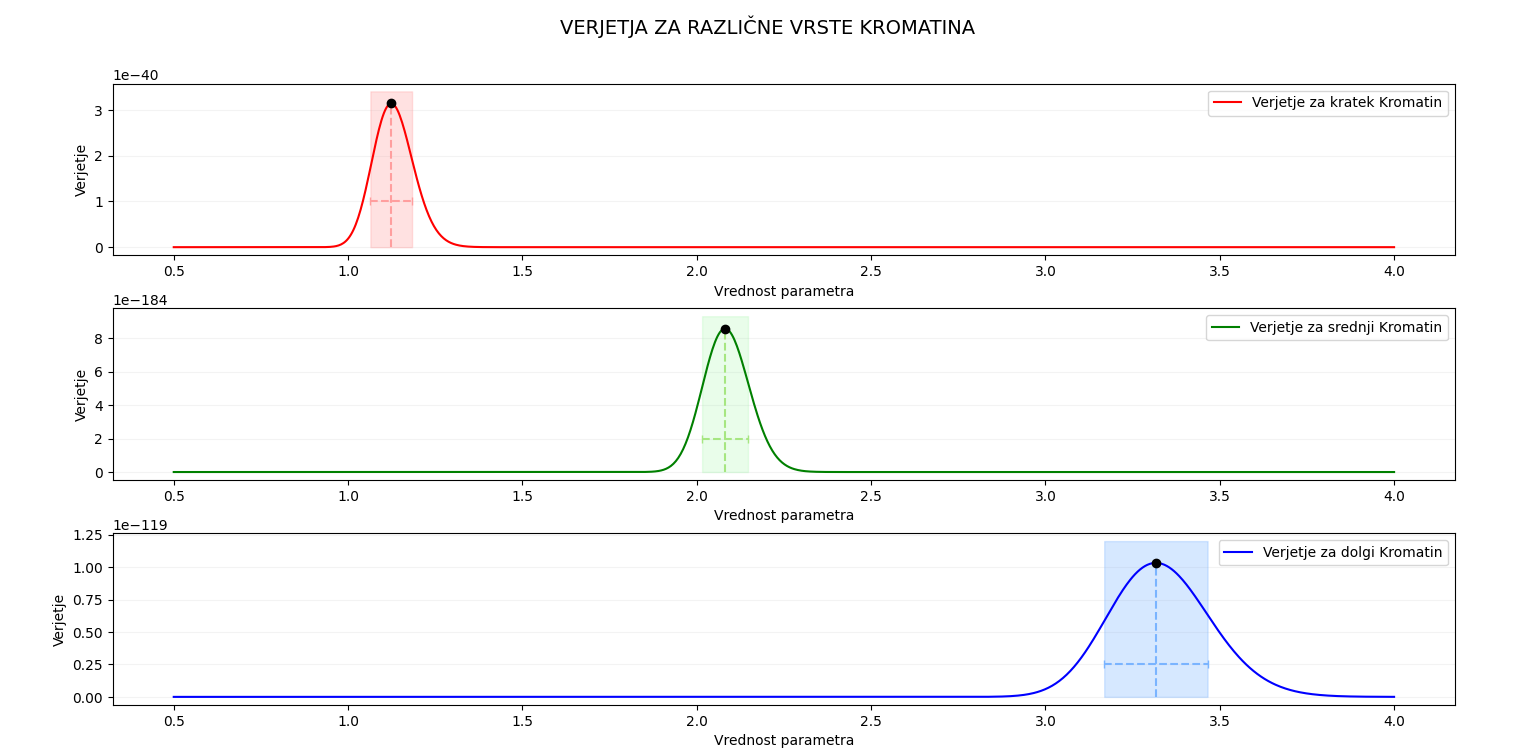
\includegraphics[width=\linewidth]{naloga2d.png}
    \vspace*{-5mm}\caption{Grafi funkcij verjetja pri različnih vrstah Kromatina}
    \end{center}    
\end{figure}
%----------------------------------------------------------------
Na sliki so prikazani grafi funkcij verjetja posamezne vrste Kromatina, v odvisnosti od parametra modela $\theta$. Kot je zapisano v legendi, so grafi funkcij verjetja za različne vrste Kromatina različno obarvani. 
Navpična črtkasta črta pri vsaki vrsti Kromatina povezuje vrednost številske ocene za $\theta$ po metodi največjega verjetja (tiste vrste Kromatina) z vrednostjo funkcije verjetja pri dani številski oceni (točka funkcijske vrednost označena s črno piko).
Na grafu je dobro vidno tudi analitično ozadje metode največjega verjetja, za vsako vrsto Kromatina namreč grafično opazimo, da ima funkcija verjetja (za tisto vrsto Kromatina) v (oziroma blizu) številski oceni za $\theta$ stacionarno točko. 
Natančneje, opazimo, da v številski oceni zavzamemo maksimum funkcije verjetja.
\newline 
Komentirajmo še pomen velikosti (pri nas ocene) standardne napake. Funkcijo verjetja določajo (za vsako vrsto Kromatina) dani podatki (o tisti vrsti Kromatina), ki obenem v model vnašajo slučaj. 
Zaradi slučajnosti, ki jih vnašajo podatki, bi radi ocenili napako, ki se morebiti pojavi pri tem, ko iz njih konstruiramo oceno (po metodi največjega verjetja) za parameter našega modela, t.j. $\hat{\theta}_{MNV}$.
Nekoliko bolj direktno, gre v resnici za statistično vrednost, ki kvantificira, koliko se lahko ocenjena vrednost parametra razlikuje od dejanske neznane vrednosti pri ponovljenem vzorčenju.
Vrednost standardne napake, oziroma v našem primeru njena ocena, nam torej določata velikost intervala okoli naše poračunane ocene za $\theta$ po metodi največjega verjetja. Na sliki je za vsako vrsto Kromatina to tudi označeno s prosojno obarvanim območjem, pri čemer meje intervala dodatno nakazuje vodoravna črtkasta daljica. 

Vredno je omeniti tudi grafično opaženo korelacijo med položnostjo zavzetja maksimuma funkcije verjetja in velikostjo (ocene) standardne napake za pripadajočo vrsto Kromatina.
Vidno je namreč, da sta številski oceni za standardni napaki kratkega in srednjega Kromatina skoraj enaki, kar se ujema z skoraj enakima širinama$~$"hriba"$~$na vrhu katerega funkcija zavzame maksimum. 
V primerjavi s kratkim in srednjim Kromatinom, je številska ocena za standardno napako pri dolgem Kromatinu večja. 
Prav tako hitro vidimo, da pri grafu verjetja za dolgi Kromatin maksimum zavzamemo nekoliko bolj položno oziroma je širini že omenjenega$~$"hriba"$~$vidno večja.
Opaženo je v resnici iz teoretičnega vidika pričakovano že iz zgornje interpretacije vrednosti standardne napake. 
\newline
\newline
Sedaj se lotimo podnaloge e). Že zgoraj omenjena $python$ datoteka nam poda številske ocene tudi za $\theta$ po metodi momentov. 
Te znašajo $1.1706$ za kratek Kromatin, $2.0748$ za srednji Kromatin in $3.4045$ za dolgi Kromatin.
Oceno za napako iščemo na podoben način, kot smo to storili pri metodi največjega verjetja. Tokrat bo številska ocena za $\theta$ tista iz metode momentov, faktor pred napako pa ustrezno drugačen. Natančneje, za oceno uporabimo:
$$
    \hat{SE}(\hat{\theta}_{MM}) = \sqrt{\frac{4 - \pi}{\pi n}} \cdot\hat{\theta}_{MM}.
$$
Številske ocene znašajo $0.06245$ za kratek Kromatin, $0.068731$ za srednji Kromatin in $0.154895$ za dolgi Kromatin.
\newline
Opazimo, da so številske vrednosti ocen standardnih napak (za $\theta$ po metodi momentov in po metodi največjega verjetja) pri enaki vrsti Kromatina skoraj enake. 
Slednje je seveda razumljivo, saj smo za oceno standardne napake vzeli koren asimptotične ocene srednje kvadratične napake, pri čemer smo $\theta$ nadomestili z glede na metodo določeno cenilko. 
Ker nam metoda največjega verjetja asimptotične daje boljšo cenilko, je tudi ocena za standardno napako, pridobljena prek te metode manjša. 
Pomen (ocene) standardne napake je enak tistemu, ki smo ga komentirali na začetku obravnave metode največjega verjetja.
Če le ponovimo, gre za vrednost, ki meri/nam pomaga razumeti, kako se ocenjena vrednost parametra lahko razlikuje od dejanske neznane vrednosti pri ponovljenem vzorčenju.
\newline
\newline
Podatke znotraj vrste Kromatina sedaj predstavimo še s histogramom. Pri tem določimo širino bloka oziroma število blokov histograma s pomočjo modificiranega Freedman–Diaconisovega pravila. 
Ta nam prek medkvartilnega razmika določi optimalno širino blokov histograma. Omenjena optimalna širina bloka pri kratkem Kromatinu znaša $0.4685$, za srednji Kromatin $0.7976$, za dolgi Kromatin pa $1.4145$.
Zapisane vrednosti širine blokov, se glede na razpon podatkov najbolje ujemajo (najbližje naravno število) s $7$ bloki pri kratkem Kromatinu, s $7$ bloki pri srednjem Kromatinu in z $8$ bloki pri dolgem Kromatinu. 
Za vsako vrsto Kromatina, na pripadajoč histogram (določen s zgoraj zapisanim številom blokov) dorišimo še pripadajoči oceni za gostoti, ki smo jo dobili iz ocene za $\theta$ po metodi momentov in po metodi največjega verjetja. 
\begin{figure}[H]
    \begin{center}
    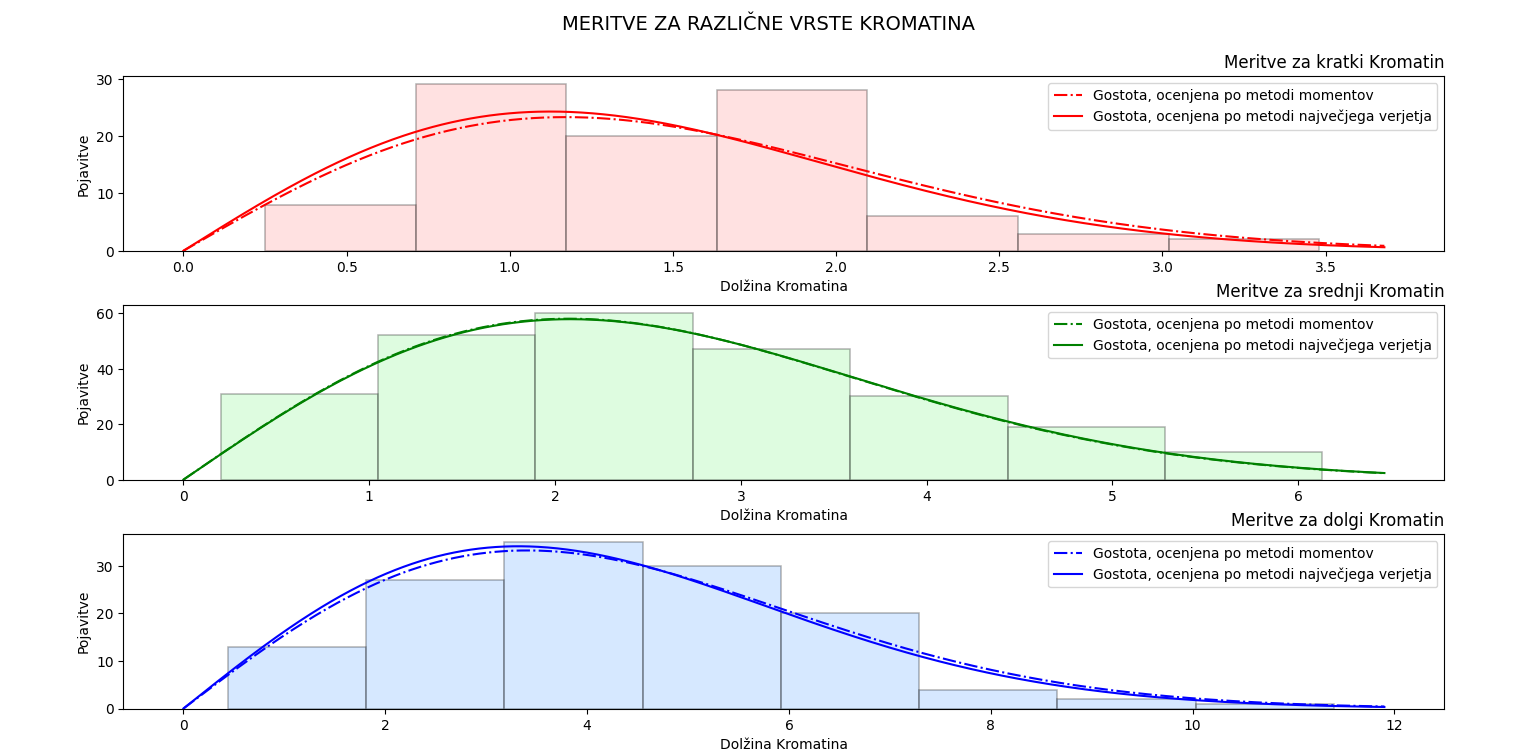
\includegraphics[width=\linewidth]{naloga2f.png}
    \vspace*{-5mm}\caption{Histogrami in ocenjene gostote za različne vrste Kromatina}
    \end{center}    
\end{figure}
Kot je to zapisano že v legendi, sta gostoti na pripadajočem histogramu dorisani z barvno usklajeno črto, tip katere pa se razlikuje glede na metodo, ki nam je omogočala izračun ocene gostote.
Vredno je omeniti, da gre za prikaz skaliranih (množili smo s skupno površino histograma) gostot, saj bomo le na ta način lahko smiselno komentirali prileganje. 
\newline
Sedaj zapišimo nekaj splošnih opazk.
Pri histogramu za srednji Kromatin opazimo, da se grafa ocen gostot skoraj ujemata, obenem pa se (izmed vseh vrst Kromatina) oceni gostot najbolj prilegata podatkom, predstavljenim s histogramom. 
Skorajšno prekrivanje ocen gostot na omenjenem grafu, je posledica bližine vrednosti za oceno cenilke obeh metod ($2.0748$ pri metodi momentov,  in $2.0812$ pri metodi največjega verjetja).
Oceni za gostoti se pri dolgem Kromatinu dokaj dobro ujemata z obliko histograma okoli vrednosti $4$, ter v desnem robu prikaza, drugod pa se obe gostoti minimalno odmakneta od histograma. 
Nekoliko manj smo lahko navdušeni nad ujemanjem grafov gostot s histogramom pri podatkih kratkega Kromatina. Tu je pomanjkanje ujemanja nekoliko posledica tudi tega, da pri izbiri števila blokov za ta primer število zaokrožimo navzgor.
Če število blokov za ta primer ročno zmanjšamo za $1$, pridemo do nekoliko lepšega ujemanja, vidnega na spodnji sliki.
\begin{figure}[H]
    \begin{center}
    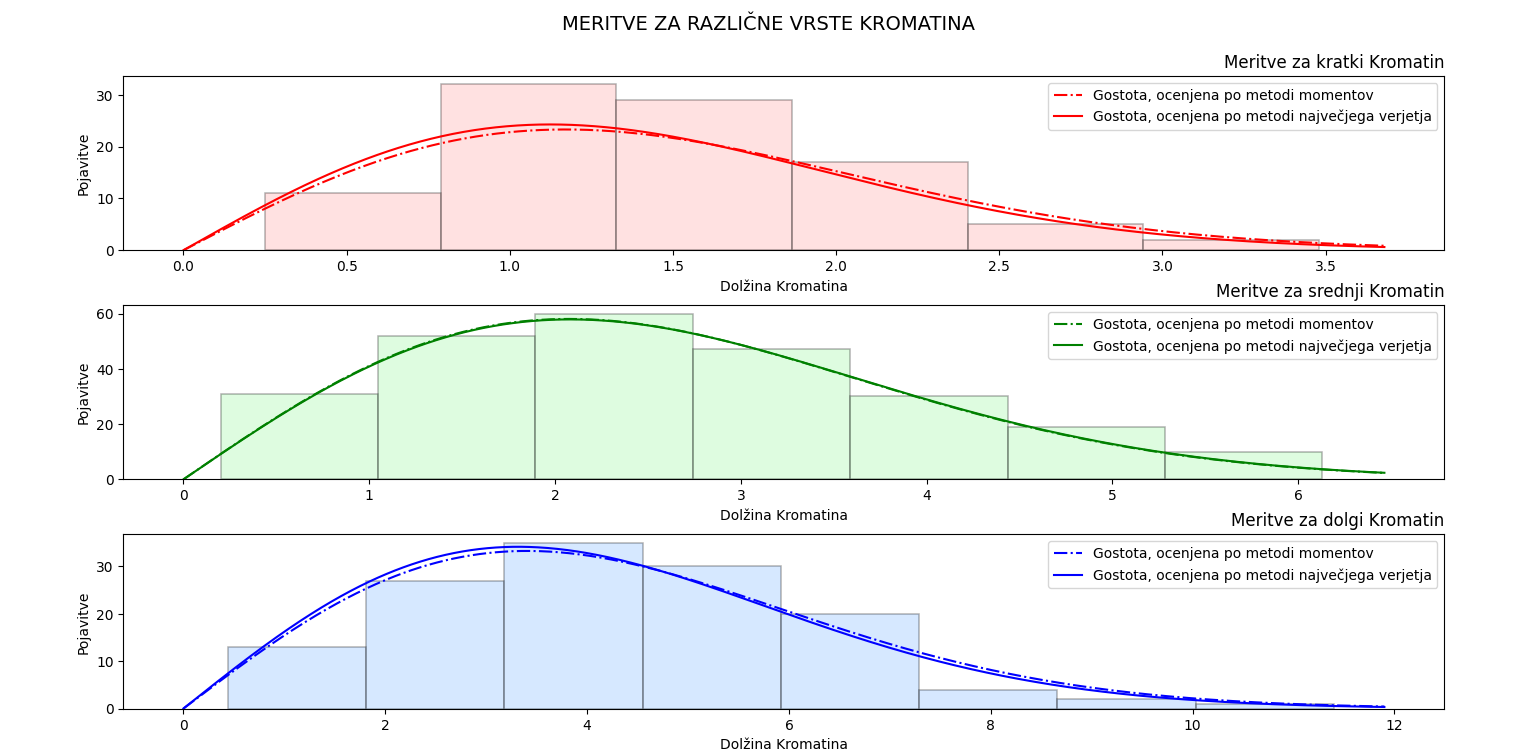
\includegraphics[width=\linewidth]{naloga2ff.png}
    \vspace*{-5mm}\caption{Popravljen histogram za kratek Kromatin}
    \end{center}    
\end{figure}
Opazimo, da je tako nekoliko manj neujemanja, moteče je le pomanjkanje podatkov histograma na levem delu grafa, ter zato presežek podatkov na sredini histograma. 
Kljub temu smo lahko nad ujemanjem gostot (med seboj) in histograma pri vseh vrstah Kromatina zadovoljni in lahko trdimo, da so rezultati razumni.

\pagebreak

\section{Naloga 3}
Naloga nam pove, da imamo podane mesečne temperature (torej $12$ podatkov letno) za $n$ zaporednih let (v našem primeru podatki med letoma $1986$ in $2020$, torej $n = 35$).
Smiselno je podatke o meritvah zapisati kot urejene pare, da se bomo lahko problema lotili z linearno regresijo.
Opažene meritve so smiselno časovne urejene (leto-mesec), zato si podatke lahko predstavljamo kot pare $(x_i,~y_i)_{i=1,~2,~\dots,~12n}$, kjer $x_i$ predstavlja časovno komponento problema, $y_i$ pa opaženo temperaturo pri časovno $i$-ti meritvi. 
V resnici lahko le pretvorimo podatek oblike: $(leto,~mesec,~temperatura)$ v par $(leto + mesec/12,~temperatura)$.
Lotimo se najprej podnaloge a), z enostavno linearno regresijo.
Označimo:
$$
    X = \begin{bmatrix}
        1 & x_1\\ 
        1 & x_2 \\
        \vdots & \vdots\\ 
        1 & x_{12n}
    \end{bmatrix}, ~
    Y = \begin{bmatrix}
        y_1 \\ 
        y_2 \\
        \vdots \\ 
        y_{12n}
    \end{bmatrix}~\text{in}~ 
    \beta = \begin{bmatrix}
        \beta_0 \\ 
        \beta_1
    \end{bmatrix}.   
$$

V duhu enostavne linearne regresije iščemo $\beta_0$ in $\beta_1$, tako da se bo $X \beta$ po metodi najmanjših kvadratov najbolje prilegal $Y$.
Teorija nam pove, da lahko $\beta$ ocenimo s cenilko:
$$
    \hat{\beta} = \Big(X^{T}X\Big)^{-1}X^{T}Y.
$$
Podane podatke bomo sedaj obdelali s pomočjo datoteke $statistika\_naloga\_3.py$. 
Konstruiramo zgoraj definirane matrike in po formuli za $\hat{\beta}$ poračunamo tudi številsko oceno za $\beta$. Ta pri danih podatkih za $\beta_0$ znaša $-125.5905$, za $\beta_1$ pa znaša $0.068303$.
\newline
Številska ocena za $\beta_1$ je za nas (iz vidika podnaloge a)) nekoliko bolj zanimiva, saj njena vrednost opisuje (glede na podatke) opažen linearen trend (v tem primeru zaradi pozitivnosti številske ocene) naraščanja temperature skozi leta.
Ta nam nakazuje, da se v povprečju temperatura letno dvigne za $0.068303$ stopinje. 
Podatki so grafično predstavljeni na spodnji sliki. 
\begin{figure}[H]
    \begin{center}
    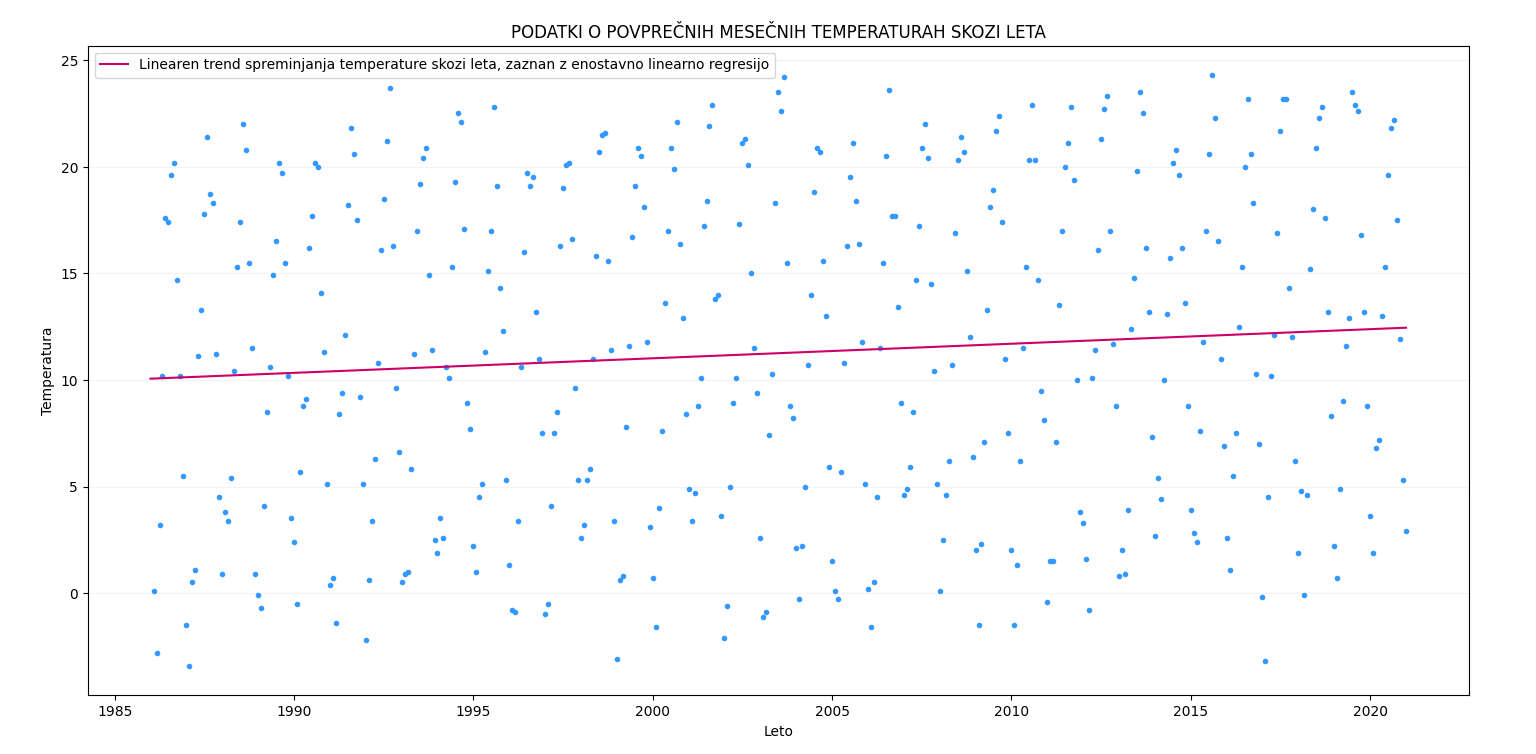
\includegraphics[width=\linewidth]{naloga3a.png}
    \vspace*{-5mm}\caption{Temperature skozi leta in linearen trend enostavne linearne regresije}
    \end{center}    
\end{figure}

Vseeno z opazkami, predvsem o naraščujočem linearnem trendu, ravnajmo nekoliko bolj previdno. 
Oglejmo si, ali je opisan linearen trend spreminjanja temperature s časom statistično značilen. 
\newline
\newline
KAJ SPLOH JE TO ??? 
\newline

Drugega dela (podnaloge b)) se lotimo z modifikacijo prvega dela. Želimo konstruirati model, ki bo vključeval tudi letno nihanje temperature. 
Podatke spet obravnavamo kot pare $(x_j,~y_j)$. Definirajmo:
$$
\mathds{1}_i(x_j)= \begin{cases}
    1;~ i \equiv j~(\text{mod}~12) \\
    0;~\text{sicer}
\end{cases};~~i \in \{1,~2,~\dots,~12\},~j \in \{1,~2,~\dots,~12n\}.
$$
V resnici vsaka izmed indikatorskih funkcij predstavlja svoj (z zaporednim indeksom določen) mesec, $x_j$ pa so časovno (z letom in mesecem) urejene meritve. 
Opazimo, da je vrednost indikatorske funkcije za nek mesec na meritvi neničelna (enaka $1$) natanko tedaj, ko je bila meritev opravljena v mesecu, ki določa indikatorsko funkcijo.
Indikatorske funkcije nam bodo omogočale zamik podatkov vsakega meseca tako, da bomo upoštevali nihanje temperature znotraj leta. 
Vredno je poskusiti z modelom oblike:
$$
    y_j = \beta_0 x_j + \sum_{i=1}^{12}{\beta_{i}~\mathds{1}_i(x_j)} + \epsilon_j,~j \in \{1,~2,~\dots,~12n\}.
$$
Zapisan model si v resnici lahko predstavljamo kot posplošitev modela iz prve podnaloge, z različno vrednostjo konstantne člena za podatke vsakega meseca. 
\newline
\newline
Sedaj lahko zapišimo v  matrični obliki in postopajmo prek postopka za linearno regresijo. 
$$
X= \left[\begin{array}{c:ccccc}
    x_1 & 1 & 0 & 0 & \dots & 0 \\
    x_2 & 0 & 1 & 0 & \dots & 0 \\
    x_3 & 0 & 0 & \ddots & & \vdots \\
    \vdots & \vdots & \vdots & & \ddots & \vdots \\
    x_{n} & 0 & 0 & 0 & \dots & 1 \\
    \hdashline
    x_{n+1} & 1 & 0 & 0 & \dots & 0 \\
    x_{n+2} & 0 & 1 & 0 & \dots & 0 \\
    x_{n+3} & 0 & 0 & \ddots & & \vdots \\
    \vdots & \vdots & \vdots & & \ddots&\vdots \\
    x_{2n} & 0 & 0 & 0 & \dots & 1\\
    \hdashline
    \vdots & \vdots & \vdots & \vdots & \dots&\vdots\\
    \hdashline
    x_{11n+1} & 1 & 0 & 0 & \dots & 0 \\
    x_{11n+2} & 0 & 1 & 0 & \dots & 0 \\
    x_{11n+3} & 0 & 0 & \ddots & & \vdots \\
    \vdots & \vdots & \vdots & & \ddots&\vdots \\
    x_{12n} & 0 & 0 & 0 & \dots & 1 \\
\end{array}\right], ~
    Y = \begin{bmatrix}
        y_1 \\ 
        y_2 \\
        \vdots \\ 
        y_{12n}
    \end{bmatrix}~\text{in}~ 
    \beta = \begin{bmatrix}
        \beta_0 \\ 
        \hdashline
        \beta_1 \\ 
        \vdots \\ 
        \beta_{12}
    \end{bmatrix}.   
$$
Podatke spet vnesemo v zgoraj omenjeno $python$ datoteko, ki nam (po formuli za cenilko $\hat{\beta}$) vrne številske ocene za posamezne koordinate $\beta$.
Številska vrednost ocene v našem primeru za $\beta_0$ znaša $0.064636$, za preostale koordinate pa dobimo številske ocene:
\begin{equation*}
\begin{split}
    \hat{\beta}_1 &= -128.6196,~\hat{\beta}_2 = -126.9164,~\hat{\beta}_3 = -122.6018,~\hat{\beta}_4 = -118.0643,\\
    \hat{\beta}_5  &= -113.4983,~\hat{\beta}_6 = -109.8351,~\hat{\beta}_7 = -107.8233,~\hat{\beta}_8 = -108.3830,\\
    \hat{\beta}_9 &= -113.4112,~\hat{\beta}_{10} = -118.1481,~\hat{\beta}_{11} = -123.4162,~\hat{\beta}_{12} = -128.2103.
\end{split}
\end{equation*}
Opazimo, da se vrednosti številskih ocen za $\beta_1,~\beta_2,~\dots,~\beta_{12}$ gibljejo okoli vrednosti iz prejšnega primera (enostavna linearna regresija, kjer je bila vrednost številske ocene za $\beta_1$ enaka $-125.5905$). 
To je bilo seveda za pričakovati, saj kot smo že omenili, gre pri vrednostih $\beta_1,~\beta_2,~\dots,~\beta_{12}$ le za prek meseca določeno konstanto (mesecu pripada njegova zaporedna številka, zaporedni številki pa pripadajoča zaporedna koordinatna ocena za $\beta$), v primeru enostavnega slučajnega vzorčenja, pa je $\beta_1$ predstavljala konstanto, določeno ne glede na mesec (torej za vse mesece hkrati). 
Vredno je omeniti tudi, da so konstante pri tipično bolj toplih mesecih (na primer maj-$5$, junij-$6$, julij-$7$) nekoliko večje, pri tipično nekoliko hladnejših mesecih (na primer november-$11$, december-$12$, januar-$1$), pa nekoliko manjše.
Zgoraj omenjene opazke, se ujemajo z intuicijo spreminjanja temperature skozi leto in nakazujejo ustrezno posplošitev modela enostavne linearne regresije na model, ki upošteva tudi letno nihanje temperature. 
\newline
Sedaj si oglejmo linearen trend spreminjanja temperature (skozi leta), v tako zastavljenem modelu. V ta namen se osredotočimo na številsko vrednost ocene za $\beta_0$. Ta je dokaj blizu številski vrednosti ocene za $\beta_0$ iz enostavne linearne regresije (v tem modelu dobimo oceno, ki znaša $0.064636$, v modelu enostavne linearne regresije pa $0.068303$). 
Novejši model nam torej nakazuje nekoliko položneje naraščajoč linearen trend spreminjanja temperature, oziroma ocenjuje, da se temperatura letno dvigne povprečno za $0.064636$ stopinje.
\newline
\newline 
P VREDNOSTI ??
\newline
\newline
Lotimo se sedaj napovedovanja novih vrednosti, oziroma po željah naloge, napovedovanj temperatur v letu $2040$. Predpostavimo, da je model Gaussov, oziroma, da so šumi, ki so vključeni v model porazdeljeni normalno ($\sim N(0,~\sigma^2)$), ter da so šumi pri prihajajočih mesecih neodvisni od preostalih šumov. 
\newline
Iz teorije vemo, da je osnova za napovedovanja naslednje vrednosti pri Gaussovem modelu linearne regresije zapis:
$$
y_{m+1} = x_{m+1,1}\beta_1 + x_{m+1,2}\beta_ + \dots + x_{m+1,p}\beta_p + \epsilon_{m+1}.
$$
Ta je naveden na četrti strani \cite{lin_reg}, kjer si je možno ogledati tudi nekoliko več matematičnega ozadja in nadaljno izpeljavo intervala zaupanja za takšno napovedovanje naslednje vrednosti. 
Izpeljavo bom tu izpustil, ter jo le apliciral na primerih, ki jih od nas zahteva naloga.
\newline
V modelu, ki upošteva nihanje letne temperature, smo se že dokopali do vrednosti cenilke za $\beta$, oziroma že poznamo številsko vrednost $\hat{\beta}$. 
Za cenilko temperature januarja $2040$ je zato smiselno vzeti kar $c_1^T \hat{\beta}$, kjer s $c_1$ označujemo:
$$
    c_1= \begin{bmatrix}
        2040 + 1/12 \\
        \hdashline
        1\\
        0\\
        \vdots\\
        0
    \end{bmatrix}.
$$
Opomnimo, da bi na enak način lahko ocenili temperaturo poljubnega meseca v letu $2040$, le $c_1$ bi morali ustrezno zamenjati za vektor $c_i$ (tu naj $i$ označuje zaporedno številko meseca), ki ima na prvi komponenti vrednost $2040 + i/12$, ter enico le na $i$-ti komponenti (prve komponente nismo šteli).
Če bi želeli zamenjati leto ocene, bi $2040$ v vektorju ustrezno zamenjali z letom poizvedbe. 
Naloga nas sprašuje po številski vrednosti ocene, zato jo zapišimo.
Za mesec januar po izračunu s pomočjo datoteke znaša $3.243$.

Za konstrukcijo intervala zaupanja se skličimo na formulo/izpeljavo iz \cite{lin_reg}, ki nam pove, da:
$$
    \frac{c^T\hat{\beta} - y_{m+1}}{\hat{\sigma}_{+}\sqrt{1 + c^T(X^TX)^{-1}c}} \sim \text{Student}(m-p), 
$$
zato bo imel interval zaupanja za $\hat{y}_{m+1}$ obliko:
$$
    c^T\hat{\beta} - F^{-1}_{\text{Student}}\left(1 - \frac{\alpha}{2}\right)\widehat{SEP}_{+} < \hat{y}_{m+1} < c^T\hat{\beta} + F^{-1}_{\text{Student}}\left(1 - \frac{\alpha}{2}\right)\widehat{SEP}_{+}.
$$
V zgornjem zapisu velja:
$$
\widehat{SEP}_{+}  = \hat{\sigma}_{+}\sqrt{1 + c^T(X^TX)^{-1}c}~~~\text{in}~~~\hat{\sigma}_{+} = \frac{||Y - X\hat{\beta}||}{\sqrt{m - p}},
$$
vredno pa je omeniti še, da $m$ predstavlja število podatkov (v našem primeru $12n = 420$) $p$ pa število koeficientov v modelu (pri nas so to v modelu, ki upošteva tudi letno nihanje temperature $\beta_0,~\beta_1,~\dots,~\beta_{12}$, torej $p$ = 13).
\newline
Ker smo cenilko za januarsko temperaturo leta $2040$ zapisali kot $c_1^T \hat{\beta}$, bo interval zaupanja po zgornji formuli oblike:
$$
[c_1^T\hat{\beta} - F^{-1}_{\text{Student}}\left(1 - \frac{\alpha}{2}\right)\widehat{SEP}_{+} ,~c_1^T\hat{\beta} - F^{-1}_{\text{Student}}\left(1 + \frac{\alpha}{2}\right)\widehat{SEP}_{+} ]
$$
Sedaj se za pomoč pri izračunavi ponovno obrnemo na program $python$, pri iskanju približka vrednosti inverza Studentove porazdelitve (pri nas stopnje $420 - 13 = 407$) pa nam na pomoč priskoči internetom. 
Navodila iz začetka projektne naloge narekujejo, da moramo interval zaupanja izračunati tako pri $\alpha = 0.01$, kot tudi pri $\alpha = 0.05$. 
Izračuni nam povedo, da stopnji tveganja $0.05$ pripada interval zaupanja $[-0.1607,~6.6466]$, pri stopnji tveganja $0.01$ pa je interval zaupanja pričakovano nekoliko večji in je $[-1.238,~7.7239]$.




Podobno se lotimo ocenjevanja povprečne temperature za leto $2040$. Za cenilko bomo vzeli kar aritmetično sredino cenilk mesecev leta $2040$, t.j.:
$$
\frac{1}{12}\sum_{i=1}^{12}{c_i^T \hat{\beta}},~\text{kjer}~c_i~\text{predstavlja ustrezne podatke za $i$ ti mesec v letu $2040$}. 
$$
Zgornjo cenilko za povprečno temperaturo leta $2040$ lahko zapišemo tudi kot $\tilde{c}^{T} \hat{\beta}$, kjer je:
$$
\tilde{c} = \begin{bmatrix}
    \frac{1}{12}\sum_{i=1}^{12}{(2040 + i/12)}\\
    1/12\\
    1/12\\
    \vdots\\
    1/12
\end{bmatrix}=
\begin{bmatrix}
    2040 + \frac{1}{144}\sum_{i=1}^{12}{i}\\
    1/12\\
    1/12\\
    \vdots\\
    1/12
\end{bmatrix}=
\begin{bmatrix}
    2040 + \frac{13}{24}\\
    1/12\\
    1/12\\
    \vdots\\
    1/12
\end{bmatrix}.
$$
Številska vrednost zgoraj zapisane ocene znaša $13.6482$, kar je torej naša ocena povprečne temperature v letu $2040$.
\newline
Določimo še intervala zaupanja za oceno povprečne temperature v letu $2040$. Postopamo po enakem postopku, kot smo to storili zgoraj, le da tokrat $c_1$ zamenja $\tilde{c}$, torej bo interval zaupanja oblike:
$$
[\tilde{c}^T\hat{\beta} - F^{-1}_{\text{Student}}\left(1 - \frac{\alpha}{2}\right)\widehat{SEP}_{+} ,~\tilde{c}^T\hat{\beta} - F^{-1}_{\text{Student}}\left(1 + \frac{\alpha}{2}\right)\widehat{SEP}_{+} ].
$$
Številske vrednosti intervala so pri stopnji tveganaj 0.05 enake $[10.2445,~17.0519]$, pri stopnji tveganja $0.01$ pa $[9.1672,~18.1292]$.








\bibliographystyle{siam}
\begin{thebibliography}{9}
    \bibitem{lin_reg}
        M. Raič \emph{Zapiski predavanj - Statistično sklepanje pri Gaussovi linearni regresiji} [ogled 5.~7.~2023], dostopno na \url{https://ucilnica.fmf.uni-lj.si/pluginfile.php/135057/mod_resource/content/2/Regresija_sklepanje.pdf}.
    \bibitem{poj_nepo_var}
        M. Raič \emph{Zapiski predavanj - Izražava povprečja in variance pri podatkih, organiziranih po skupinah} [ogled 3.~7.~2023], dostopno na \url{https://ucilnica.fmf.uni-lj.si/pluginfile.php/135261/mod_resource/content/2/Razcep_var.pdf}.
\end{thebibliography}

\end{document}